\section{Graph definitions and terminology}
\begin{definitionBox}[Directed graphs]
    A directed graph consists of a set of vertices and a set of directed edges that connect pairs of vertices.

    In probability, the vertices are random variables. Figure~\ref{fig:simple_dag} shows an example of a directed graph.
\end{definitionBox}
\begin{definitionBox}[Directed acyclic graph]
    \label{def:directed acyclic graph}
    A directed acyclic graph (DAG) is a directed graph that contains no cycles. That is, no directed paths from a vertex back to itself.

    In case of probability, a DAG is called a \emph{Bayesian network} (BN).
\end{definitionBox}

\begin{figure}[h]
    \centering
    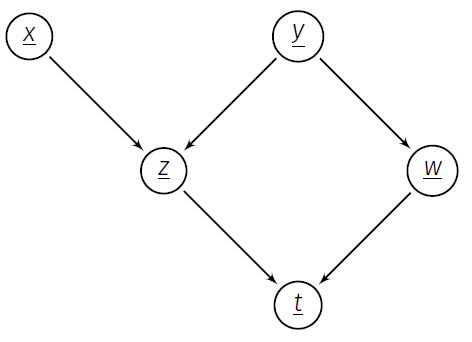
\includegraphics[width=0.4\textwidth]{figs/Graphs/simple_dag.PNG}    
    \caption{Illustration of a simple directed graph in probability.}
    \label{fig:simple_dag}
\end{figure}

% \subsubsection{Terminology}
The terms are illustrated in the figures below. 
\begin{figure}[H]
    \centering
    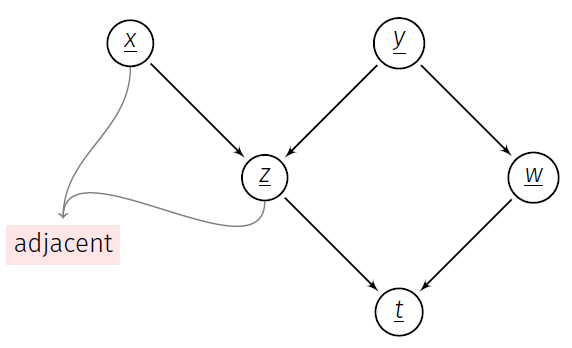
\includegraphics[width=0.4\textwidth]{figs/Graphs/dag_adjacent_vertices.PNG}    
    \caption{Directed graph terminology: adjacent vertices.}
    \label{fig:dag_adjacent_vertices}
\end{figure}
\begin{figure}[H]
    \centering
    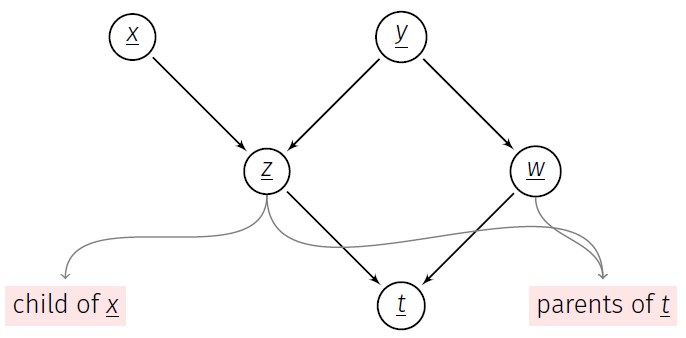
\includegraphics[width=0.4\textwidth]{figs/Graphs/dag_child_and_parent.PNG}    
    \caption{Directed graph terminology: child and parent vertices.}
    \label{fig:dag_child_and_parent}
\end{figure}
\begin{figure}[H]
    \centering
    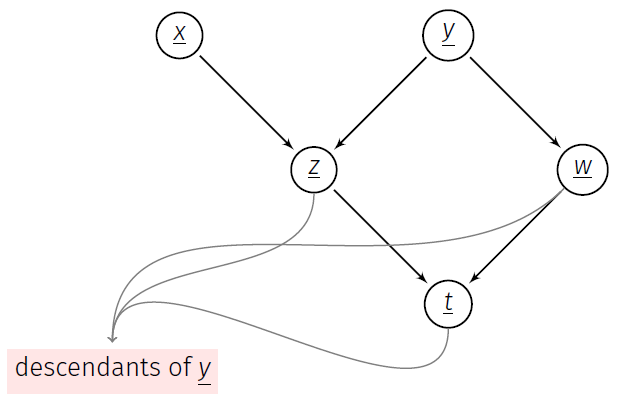
\includegraphics[width=0.4\textwidth]{figs/Graphs/dag_descendents.PNG}    
    \caption{Directed graph terminology: descendants vertices.}
    \label{fig:dag_descendents}
\end{figure}
\begin{figure}[H]
    \centering
    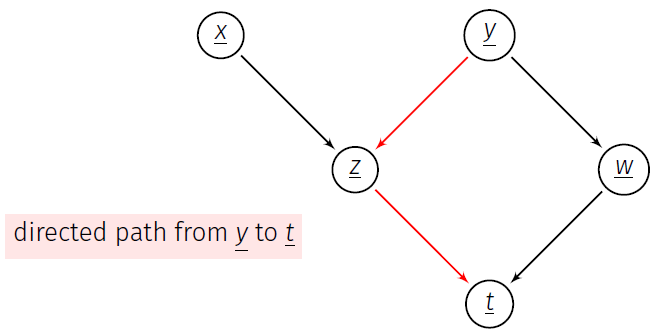
\includegraphics[width=0.4\textwidth]{figs/Graphs/dag_directed_path.PNG}    
    \caption{Directed graph terminology: directed path.}
    \label{fig:dag_directed_path}
\end{figure}
\begin{figure}[H]
    \centering
    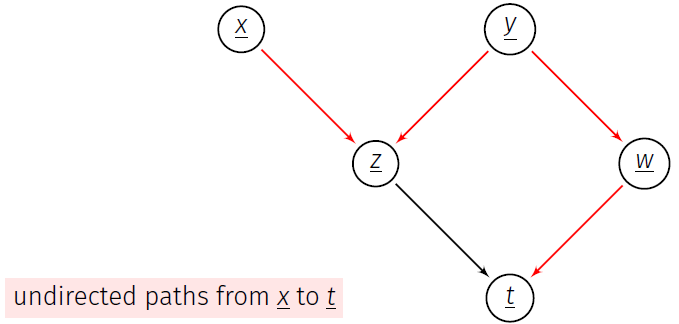
\includegraphics[width=0.4\textwidth]{figs/Graphs/dag_undirected_path.PNG}    
    \caption{Directed graph terminology: undirected path.}
    \label{fig:dag_undirected_path}
\end{figure}
\begin{figure}[H]
    \centering
    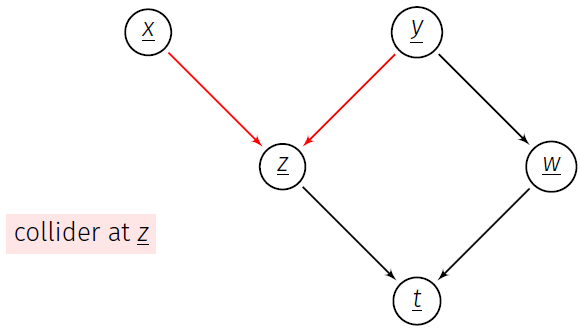
\includegraphics[width=0.4\textwidth]{figs/Graphs/dag_collider.PNG}    
    \caption{Directed graph terminology: collider.}
    \label{fig:dag_collider}
\end{figure}

\section{Graphs in Probability}
\begin{definitionBox}[Bayesian networks]
    A Bayesian network is a directed acyclic graph (DAG) (check Def.~\ref{def:directed acyclic graph}) that has random variables as vertices.
\end{definitionBox}

\begin{mytheorem}
   [Representing JPDFs using DAGs]    
   {Representing JPDFs using DAGs}
   Consider $n$ random variables $\rv{x}_{1}, \ldots, \rv{x}_{n}$ with joint pdf (JPDF) $\pdf{x_{1},\ldots,x_{n}}$. Let $G$ be a DAG with $n$ vertices representing the random variables. Then, $G$ represents the JPDF $\pdf{}$ if 
   \begin{align}
    \pdf{x_{1}, \ldots, x_{n}} &= \prod_{i=1}^{n} \pdf{x_{i}\middle|~ \text{parents of } x_{i}}.
\end{align}
\end{mytheorem}

\begin{mytheorem}
   [Markov condition in DAG]    
     The DAG $G$ represents the JPDF $\pdf{}$ if and only if the Markov condition holds, which states the following:
     \begin{align}        
         \forall \rv{x}_{i} : \quad \rv{x}_{i} \perp \bar{\mc{X}}_{i} | \text{parents of } \rv{x}_{i},
     \end{align}
     where $\bar{\mc{X}}_{i}$ are all other random variables but the parents and descendants of $\rv{x}_{i}$.
\end{mytheorem}

\begin{definitionBox}[D-donnection and d-separation]
    Consider a set of $n$ random variables $\rv{x}_{1}, \ldots, \rv{x}_{n}$ whose JPDF is represented by $G$. 
    Furthermore, let $\mc{A}$, $\mc{B}$, and $\mc{C}$ be mutually exclusive sets with $\mc{A},\mc{C}\neq\emptyset$.

    The sets $\mc{A}$ and $\mc{C}$ are called \emph{d-connected} given $\mc{B}$ if there exists an \emph{undirected} path between some random variable in $\mc{A}$ and some random variable in $\mc{C}$ such that 
    \begin{enumerate}
        \item every collider along the path is in $\mc{B}$, or has a descendent in $\mc{B}$;
        \item no non-collider along the path belongs in $\mc{B}$.
    \end{enumerate}
    If $\mc{A}$ and $\mc{C}$ are not d-connected given $\mc{B}$, then they are called \emph{d-separated given $\mc{B}$}.
\end{definitionBox}

\begin{mytheorem}
   [D-connection and d-separation] 
   Consider a set of $n$ random variables $\rv{x}_{1}, \ldots, \rv{x}_{n}$ whose JPDF is represented by $G$. Furthermore, let $\mc{A}$, $\mc{B}$, and $\mc{C}$ be mutually exclusive sets with $\mc{A},\mc{C}\neq\emptyset$. Then, 
     the sets $\mc{A}$ and $\mc{C}$ are \emph{d-separated given} $\mc{B}$ if and only if 
     \begin{align}
         \mc{A} \perp \mc{C} | \mc{B}.
     \end{align}
\end{mytheorem}